% -*- latex -*-
%%%%%%%%%%%%%%%%%%%%%%%%%%%%%%%%%%%%%%%%%%%%%%%%%%%%%%%%%%%%%%%%
%%%%%%%%%%%%%%%%%%%%%%%%%%%%%%%%%%%%%%%%%%%%%%%%%%%%%%%%%%%%%%%%
%%%%
%%%% This text file is part of the source of 
%%%% `Parallel Computing'
%%%% by Victor Eijkhout, copyright 2012-5
%%%%
%%%% mpi-started.tex : introductory chapter about MPI
%%%%
%%%%%%%%%%%%%%%%%%%%%%%%%%%%%%%%%%%%%%%%%%%%%%%%%%%%%%%%%%%%%%%%
%%%%%%%%%%%%%%%%%%%%%%%%%%%%%%%%%%%%%%%%%%%%%%%%%%%%%%%%%%%%%%%%

In this chapter you will learn the use of the main tool for 
distributed memory programming: the \acf{MPI} library.
The \ac{MPI} library has about 250 routines, many of which you may
never need. Since this is a textbook, not a reference manual, we will
focus on the important concepts and give the important routines for
each concept. What you learn here should be enough for most common
purposes. You are advised to keep a reference document handy, in
case there is a specialized routine, or to look up subtleties about
the routines you use.

\Level 0 {Distributed memory and message passing}

In its simplest form, a distributed memory machine is a collection of
single computers hooked up with network cables. In fact, this has a name:
a \indexterm{Beowulf cluster}. As you recognize from that setup, 
each processor can run an independent program, and has its own memory
without direct access to other processors' memory. MPI is the magic
that makes multiple instantiations of the same executable run
so that they know about each other and can exchange data through the 
network.

One of the reasons that MPI is so successful as a tool for high
performance on clusters is that it is very explicit: the programmer
controls many details of the data motion between the processors.
Consequently, a capable programmer can write very efficient code with MPI.
Unfortunately, that programmer will have to spell things out
in considerable detail. For this reason, people sometimes call MPI
`the assembly language of parallel programming'. If that sounds scary,
be assured that things are not that bad. You can get started 
fairly quickly with MPI, using just the basics,
and coming to the more sophisticated tools 
only when necessary.

Another reason that MPI was a big hit with programmers is that
it does not ask you to learn a new language: it is a library that 
can be interface to C/C++ or Fortran; there are even bindings to Python.
A~related point is that it is easy to install: there are free implementations
that you can download and install on any computer that has a Unix-like
operating system, even if that is not a parallel machine.

\Level 0 {History}

Before the MPI standard was developed in 1993-4, there were many
libraries for distributed memory computing, often proprietary
to a vendor platform. MPI standardized the inter-process communication
mechanisms. Other features, such as process management in \indexterm{PVM},
or parallel I/O were omitted. Later versions of the standard
have included many of these features.

Since MPI was designed by a large number of academic and commercial
participants, it quickly became a standard. A~few packages
from the pre-MPI era, such as \indexterm{Charmpp}~\cite{charmpp},
are still in use since they support mechanisms that do not exist
in MPI.

\Level 0 {Basic model}
\label{sec:mpiexec}

Here we sketch the two most common scenarios for using MPI. In the
first, the user is working on an interactive machine, which has
network access to a number of hosts, typically a network of workstations;
see figure~\ref{fig:mpi-interactive}.
\begin{figure}[ht]
  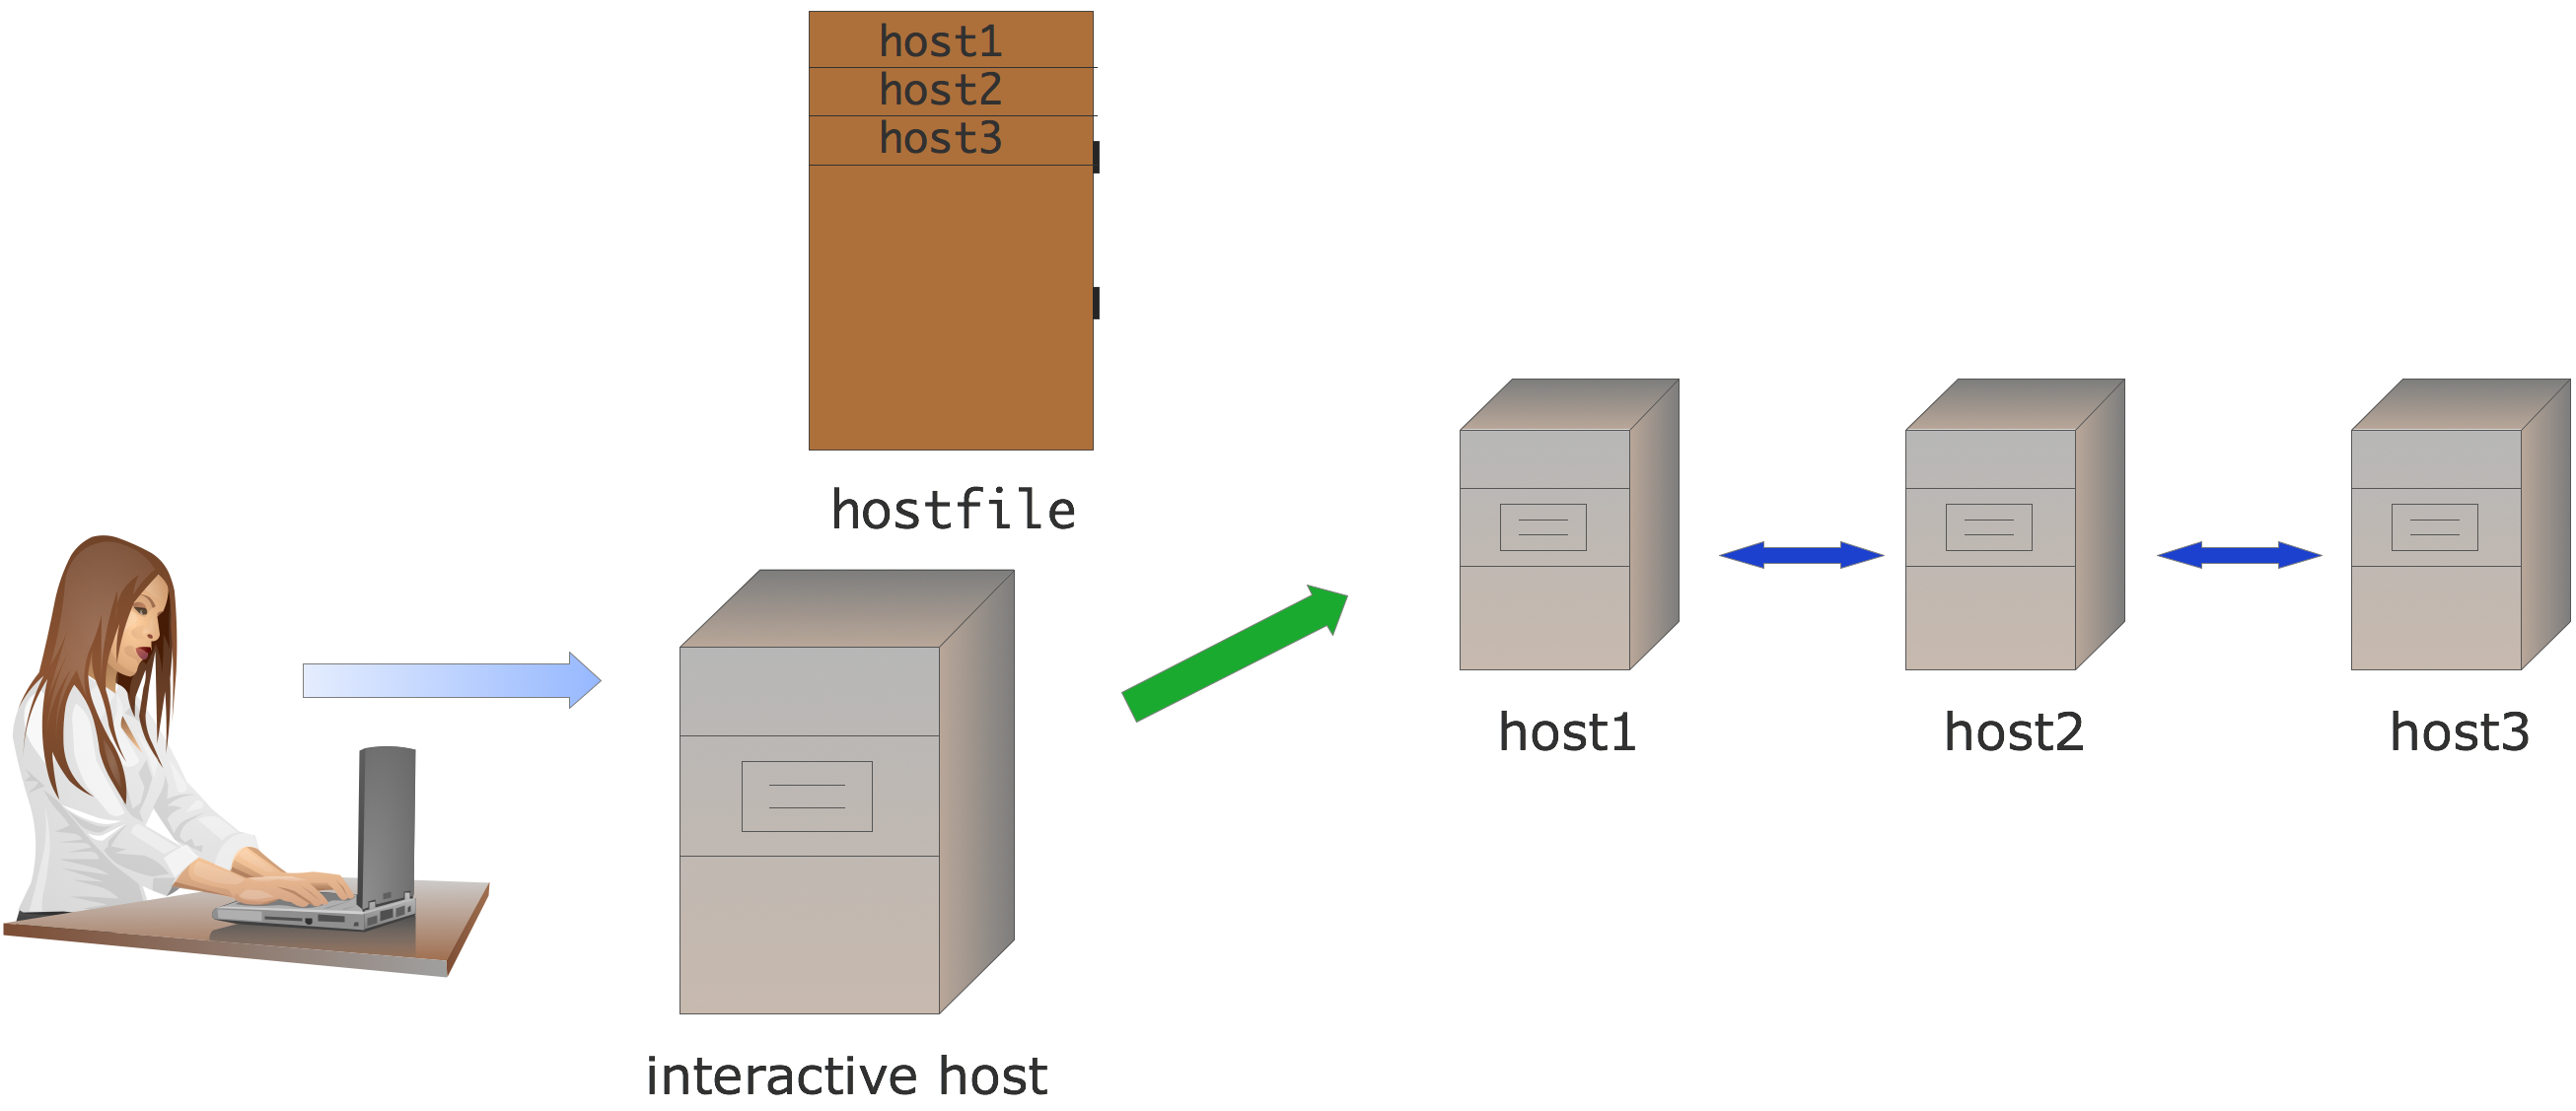
\includegraphics[scale=.12]{graphics/mpi-interactive}
  \caption{Interactive MPI setup}
  \label{fig:mpi-interactive}
\end{figure}
The user types the command \n{mpiexec}\index{mpiexec}\footnote
{A command variant is \texttt{mpirun}\index{mpirun}; your local cluster
  may have a different mechanism.}
and supplies
\begin{itemize}
\item The number of hosts involved,
\item their names, possibly in a hostfile,
\item and other parameters, such as whether to include the interactive
  host; followed by
\item the name of the program and its parameters.
\end{itemize}
The \n{mpirun} program then makes an \n{ssh}\index{ssh} connection
to each of the hosts, giving them sufficient information that they 
can find each other. All the output of the processors is piped through the 
\n{mpirun} program, and appears on the interactive console.

In the second scenario (figure~\ref{fig:mpi-batch}) the user prepares
a \indextermbus{batch}{job} script with commands, and these will be
run when the \indextermbus{batch}{scheduler} gives a number of hosts
to the job.
\begin{figure}[ht]
  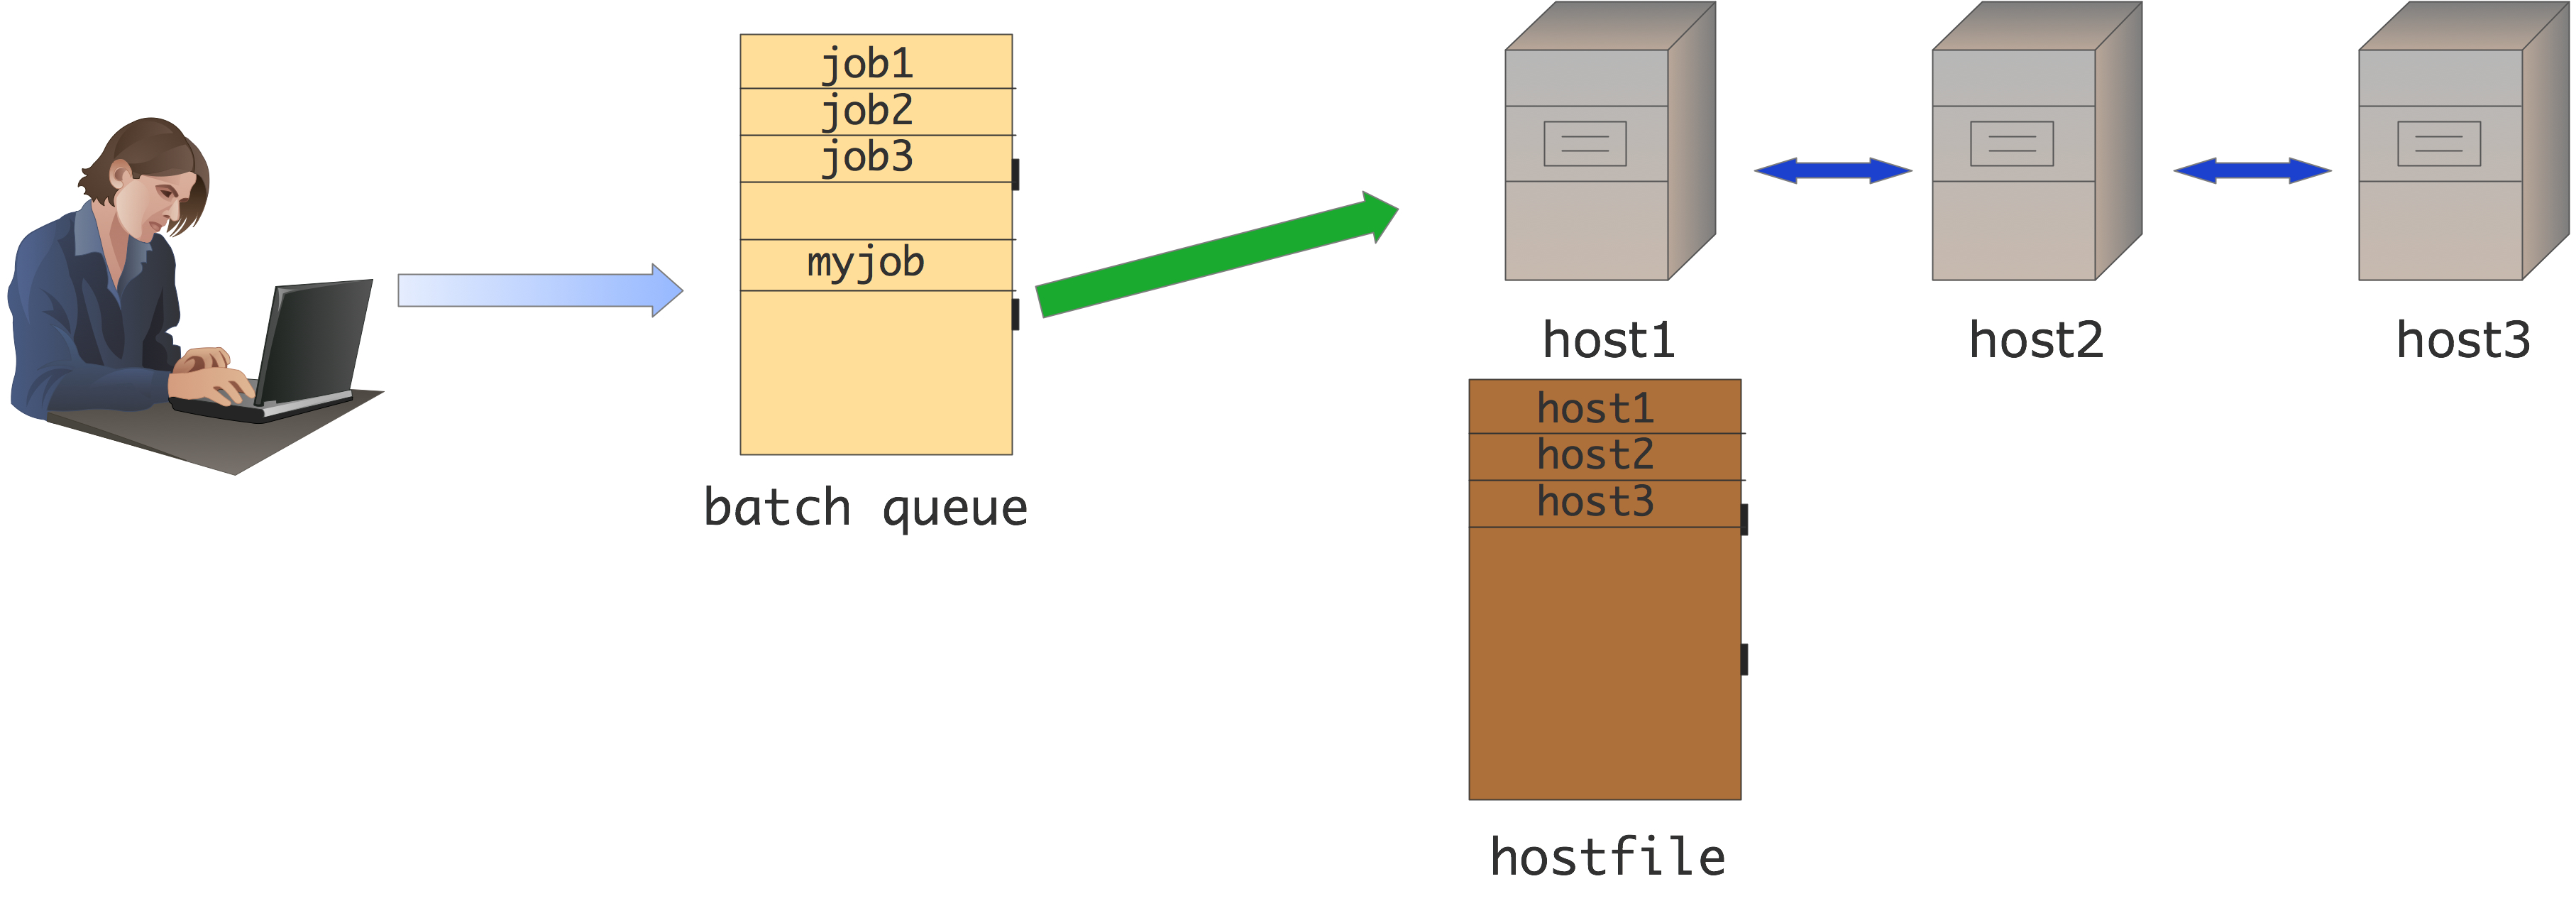
\includegraphics[scale=.1]{graphics/mpi-batch}
  \caption{Batch MPI setup}
  \label{fig:mpi-batch}
\end{figure}
Now the batch script contains the \n{mpirun} command%
\begin{istc}
, or some variant such as \n{ibrun}\index{ibrun}%
\end{istc}
, and the hostfile is dynamically generated when the job starts.
Since the job now runs at a time when the user may not be logged in, 
any screen output goes into an output file.

You see that in both scenarios the parallel program is started
by the \n{mpirun} command using
an \ac{SPMD} mode of execution: all hosts execute the same program.
It is possible for different hosts to execute different programs,
but we will not consider that in this book.

\Level 0 {Making and running an MPI program}

MPI is a library, called from programs in ordinary programming languages
such as C/C++ or Fortran. To compile such a program you use your regular
compiler:
\begin{verbatim}
gcc -c my_mpi_prog.c -I/path/to/mpi.h
gcc -o my_mpi_prog my_mpi_prog.o -L/path/to/mpi -lmpich
\end{verbatim}
However, MPI libraries may have different names between different
architectures, making it hard to have a portable makefile. Therefore,
MPI typically has shell scripts around your compiler call:
\begin{verbatim}
mpicc -c my_mpi_prog.c
mpicc -o my_mpi_prog my_mpi_prog.o
\end{verbatim}

MPI programs can be run on many different architectures. Obviously it
is your ambition (or at least your dream) to run your code on a
cluster with a hundred thousand processors and a fast network. But
maybe you only have a small cluster with
plain \indexterm{ethernet}. Or maybe you're sitting in a plane, with
just your laptop. An MPI program can be run in all these
circumstances~--~within the limits of your available memory of course.

The way this works is that you do not start your executable directly,
but you use a program, typically called \n{mpirun}\index{mpirun} or
something similar, which makes a connection to all available
processors and starts a run of your executable there. So if you have a
thousand nodes in your cluster, \n{mpirun} can start your program once
on each, and if you only have your laptop it can start a few instances
there. In the latter case you will of course not get great
performance, but at least you can test your code for correctness.

\Level 0 {Language bindings}

\Level 1 {C/C++}
\index{MPI!C/C++ bindings|see{C/C++, bindings}}
\index{C!bindings|(}
\index{C++!bindings|(}

The MPI library is written in~C. Thus, its bindings are the most natural
for that language.

C++ bindings existed at one point, but they were declared deprecated.
The \indexterm{boost} library has its own version of MPI.  A~recent
effort at idiomatic C++ support is \indexterm{MPL}
\url{http://numbercrunch.de/blog/2015/08/mpl-a-message-passing-library/}.

\index{C!bindings|)}
\index{C++!bindings|)}

\Level 1 {Fortran}

\index{Fortran!bindings|(}

The \emph{Fortran bindings} for MPI look very much like the C~ones, except that
each routine has a final \indexterm{error return} parameter.

\begin{fortrannote}
  Other Fortran-specific differences will be indicated with a note
  like this.
\end{fortrannote}

\index{Fortran!bindings|)}

\Level 1 {Python}

\index{Python!bindings|(}

The \indextermtt{mpi4py} package of \emph{python bindings}
is not defined by the MPI
standards committee. Instead, it is the work of an individual,
\indextermsub{Lisandro}{Dalcin}.

Notable about the Python bindings is that many communication routines
exist in two variants:
\begin{itemize}
\item a version that can send native Python objects. These routines
  have lowercase names such as \n{bcast}; and
\item a version that sends \indexterm{numpy} objects; these routines
  have names such as \n{Bcast}. Their syntax can be slightly different.
\end{itemize}
The first version looks more `pythonic', is easier to write,
and can do things like sending python objects,
but it is also decidedly less efficient since data is packed
and unpacked with \n{pickle}. As a common sense guideline,
use the \n{numpy} interface in the performance-critical parts
of your code, and the native interface only for complicated
actions in a setup phase.

Codes with \texttt{mpi4py} can be interfaced to other languages
through Swig or conversion routines.

Data in \texttt{numpy} can be specified as a simple object,
or \texttt{[data, (count,displ), datatype]}.

\index{Python!bindings|)}
